% -----------------------------------------------------------------------------
%
% Copyright (c) 2017 Sam Cox, Roberto Sommariva
%
% This file is part of the AtChem2 software package.
%
% This file is covered by the MIT license which can be found in the file
% LICENSE.md at the top level of the AtChem2 distribution.
%
% -----------------------------------------------------------------------------

\chapter{Model Execution} \label{ch:execution}

% -------------------------------------------------------------------- %
\section{Box-Model} \label{sec:box-model}

AtChem2 is designed to build and run atmospheric chemistry box-models
based upon the Master Chemical Mechanism (\href{http://mcm.leeds.ac.uk/MCM/}{MCM}).
Other chemical mechanisms can be used, as long as they are provided in
the correct format, described in Sect.~\ref{sec:chemical-mechanism}.

This chapter explains how to set up, compile and run an AtChem2
atmospheric chemistry model. A working knowledge of the \textbf{unix shell} and its
\href{https://swcarpentry.github.io/shell-novice/reference/}{basic commands}
\emph{is required} to use the AtChem2 model.

The directory structure of AtChem2 is described in
Sect.~\ref{sec:model-structure}. An AtChem2 box-model requires two
sets of inputs, which are described below: the mechanism
file and the configuration files.

\subsection{Mechanism file} \label{subsec:mechanism-file}

AtChem2 requires a chemical mechanism in
\hyperref[subsec:facsimile-format]{FACSIMILE format} (\texttt{.fac}).
The mechanism file can be downloaded from the MCM website using the
\hyperref[subsec:mcm-extraction]{extraction tool} or it can be
assembled manually. The user can edit the \texttt{.fac} file with a
text editor, if required.

The \texttt{.fac} file is converted into a shared library
(\texttt{mechanism.so}) and a number of mechanism files during the
build process, as explained in Sect.~\ref{subsec:build-process}).
These files are created in the \sharedir\ which, by default, is the
\texttt{model/configuration/} directory; the location of the
\sharedir\ can be modified by the user (Sect.~\ref{sec:build}).

\subsection{Configuration files} \label{subsec:configuration-files}

The box-model configuration is set via a number of text files,
which can be edited with a text editor: 

\begin{itemize}
\item model and solver parameters -- go to
  \hyperref[sec:model-parameters]{Model Parameters} and
  \hyperref[sec:solver-parameters]{Solver Parameters}.
\item environment variables settings -- go to
  \hyperref[sec:environment-variables]{Environment Variables}.
\item photolysis rates settings -- go to
  \hyperref[sec:photolysis-rates]{Photolysis Rates}.
\item initialization of the chemical species, model output settings -- go
  to \hyperref[sec:config-files]{Config Files}.
\end{itemize}

Detailed information on each configuration files can be found in
Chapt.~\ref{ch:setup}. By default, the configuration files are in the
\texttt{model/configuration/} directory, unless this is changed by the
user (Sect.~\ref{sec:build}).

% -------------------------------------------------------------------- %
\section{Constraints} \label{sec:constraints}

AtChem2 can be run in two modes:

\begin{itemize}
\item unconstrained: all variables are calculated by the model from
  the initial conditions, which are set in the
  \hyperref[subsec:configuration-files]{configuration files}.
\item constrained: one or more variables are constrained, meaning that
  the solver forces their value to a given value at each time
  step. The variables that are not constrained are calculated by the
  model.
\end{itemize}

The constraint data  must be provided as one file for each
constrained variable, with the format described below. By default, the
files with the constraint data are in \texttt{model/constraints/species/}
for the chemical species, \texttt{model/constraints/environment/} for
the environment variables, \texttt{model/constraints/photolysis/}
for the photolysis rates. The default directories can be changed, as
explained Sect.~\ref{sec:build} (see also Sect.~\ref{subsec:model-directory}).

\subsection{Constrained variables} \label{subsec:constrained-variables}

\subsubsection{Environment variables}

All environment variables, except \texttt{ROOF}, can be
constrained. To do so, set the variable to \texttt{CONSTRAINED} in
\texttt{environmentVariables.config} and create
a file with the constraint data (Sect.~\ref{subsec:constraint-files}). The name of the file must be the
same as the name of the variable, e.g., \texttt{TEMP} (without
extension).

\subsubsection{Chemical species}

Any chemical species in the chemical mechanism can be constrained. To
do so, add the name of the species to
\texttt{speciesConstrained.config} and create a
file with the constraint data (Sect.~\ref{subsec:constraint-files}). The name of the file must be the same
as the name of the chemical species, e.g., \texttt{CH3OH} (without
extension).

\subsubsection{Photolysis rates}

Any of the photolysis rates in the chemical mechanism can be
constrained. The photolysis rates are identified as \verb|J<n>|, where
\texttt{n} is an integer (Sect.~\ref{sec:photolysis-rates}). To
constrain a photolysis rate add its name (e.g., \texttt{J4}) to
\texttt{photolysisConstrained.config} and create
a file with the constraint data (Sect.~\ref{subsec:constraint-files}). The name of the file must be the
same as the name of the photolysis rate, e.g., \texttt{J4} (without
extension).

\subsection{Constraint files} \label{subsec:constraint-files}

The files with the constraint data are text files with two columns
separated by spaces. The first column is the time in \textbf{seconds}
from midnight of day/month/year (Sect.~\ref{sec:model-parameters}),
the second column is the value of the variable in the appropriate
unit. For the chemical species the unit is molecule cm$^{-3}$ and
for the photolysis rates the unit is s$^{-1}$; for the units of the environment
variables go to Sect.~\ref{sec:environment-variables}. For example:

\begin{verbatim}
-900   73.21
0      74.393
900    72.973
1800   72.63
2700   72.73
3600   69.326
4500   65.822
5400   63.83
6300   64.852
7200   64.739
\end{verbatim}

The time in the first column of a constraint file can be negative.
AtChem2 interprets negative times as ``seconds \emph{before} midnight
of day/month/year''. A negative time can be useful to allow correct
interpolation of the variables at the beginning of the model run. This
is because the model constraints \emph{must cover} the same amount of
time, or preferably more, as the intended model runtime. For example:
if the model starts at 42300 seconds and stops at 216000 seconds, the
first and the last data points in a constraint file must have a time
of 42300 seconds (or lower) and 21600 seconds (or higher),
respectively.

\subsection{Interpolation} \label{subsec:interpolation}

Constraints can be provided at different timescales. Typically, the
constraint data come from direct measurements and it is very common
for different instruments to sample with different frequencies. For
example, ozone and nitrogen oxides can be measured once every minute,
but most organic compounds can be measured only once every hour.

The user can average the constraints so that they are all at the same
timescale or can use the data with the original timescales. Both
approaches have advantages and disadvantages in terms of how much
pre-processing work is required, and in terms of model accuracy and
integration speed \citep{sommariva_2020}. Whether all the constraints
have the same timescale or not, the solver interpolates between data
points using the interpolation method selected in
\texttt{model.parameters} (Sect.~\ref{sec:model-parameters}). The
default interpolation method is piecewise linear, but piecewise
constant interpolation is also available.

The photolysis rates and the environment variables are evaluated by
the solver when needed -- each is interpolated individually, only when
constrained. This happens each time the function
\texttt{mechanism\_rates()} is called from \texttt{FCVFUN()}, and is
controlled by CVODE as it carries out the integration. In a
similar way, the interpolation routine for the chemical species is
called once for each of the constrained species in \texttt{FCVFUN()},
plus once when setting the initial conditions of each of the
constrained species.

As mentioned above, the model start and stop time \emph{must be}
within the time interval of the constrained data to avoid
interpolation errors or model crash. If data is not supplied for the
full runtime interval, then the \emph{final} value will be used for
all times both \emph{before the first data point} and \emph{after the
  last data point}. A warning is printed for all data evaluations
outside of the supplied time interval. This behaviour is likely to
change in future versions, at least to avoid the situation where the
last value is used for all times before the first~\footnote{See issue
\href{https://github.com/AtChem/AtChem2/issues/294}{\#294}}. In any
case, it is good practice to always provide constraint data that cover
a short time \emph{beyond} the final model time.

% -------------------------------------------------------------------- %
\section{Build} \label{sec:build}

The script \texttt{build\_atchem2.sh} in the \texttt{build/} directory
is used to process the chemical mechanism file (\texttt{.fac}) and
compile the model. The script generates one Fortran file
(\texttt{mechanism.f90}), one shared library (\texttt{mechanism.so})
and four mechanism files (\texttt{mechanism.prod},
\texttt{mechanism.reac}, \texttt{mechanism.ro2},
\texttt{mechanism.species}) in the \sharedir\ (by default, \texttt{model/configuration/}).
The content and format of these files are described in Sect.~\ref{subsec:build-process}.

The \texttt{build/build\_atchem2.sh} script must be run from the
\maindir\ and takes three arguments which must be passed in the exact
order indicated below. This means that if -- for example -- the second
argument needs to be specified, it is also necessary to specify the
first, even if it has the default value. To avoid mistakes, the user
can choose to always specify all the arguments. The four arguments,
and their default values, are:

\begin{enumerate}
\item the path to the chemical mechanism file -- no default
  (it is suggested to keep the \texttt{.fac} file in the \texttt{model/} directory).
\item the path to the \sharedir, i.e., the directory for the Fortran and mechanism files
  generated from the \texttt{.fac} file -- default:\\
  \texttt{model/configuration/}.
\item the path to the directory containing the MCM data files -- default:\\
  \texttt{mcm/}.
\end{enumerate}

For example, if the chemical mechanism file is in the \texttt{model/}
directory, the model is build using the command:

\begin{verbatim}
./build/build_atchem2.sh model/mechanism.fac model/configuration/ mcm/
\end{verbatim}

An installation of AtChem2 can have multiple \texttt{model/}
directories, corresponding to different models or different
projects; this allows the user to work with more than one model at the same
time. In the following example, the \maindir\ contains two
\texttt{model/} directories with different names (\texttt{model\_1/}
and \texttt{model\_2/}, each with their own chemical mechanism,
configuration, constraints and output:

\begin{verbatim}
AtChem2/
        | mcm/
        | model_1/
             | configuration/
             | constraints/
             | output/
             | mechanism.fac
        | model_2/
             | configuration/
             | constraints/
             | output/
             | mechanism.fac
        | obj/
        | src/
        | tools/
        | travis/
\end{verbatim}

The \texttt{model/} directories can also be located outside the
\maindir: as long as the correct paths are passed to the
\texttt{build\_atchem2.sh} script and to the exectuable (Sect.~\ref{sec:execute}),
the model will compile and run. For example:

\begin{verbatim}
./build/build_atchem2.sh model_1/mechanism.fac model_1/configuration/
./build/build_atchem2.sh model_2/mechanism.fac model_2/configuration/
\end{verbatim}

Note that the fourth argument is not specified in the example above,
so the default value (\texttt{mcm/}) will be used.

Compilation is required only once for a given \texttt{.fac} file. If
the user changes the configuration files, there is no need to
recompile the model. Likewise, if the constraints files are changed,
there is no need to recompile the model. This is because the model
configuration and the model constraints are read by the executable at
runtime. However, if the user changes the \texttt{.fac} file,
then the shared library \texttt{mechanism.so}
needs to be recompiled using the \texttt{build\_atchem2.sh} script.

The user may also want, or need, to change the Fortran code
(\texttt{src/*.f90}), in which case the model needs to be recompiled:
if the \texttt{.fac} file has also been changed, use the
\texttt{build\_atchem2.sh} script. Otherwise, if only the Fortran code
has been changed, executing \texttt{make} from the \maindir\ is enough
to recompile the model.

% -------------------------------------------------------------------- %
\section{Execute} \label{sec:execute}

The compilation process creates an executable file called
\texttt{atchem2} in the \maindir. The executable file
takes 10 arguments, corresponding to the directories containing the
model configuration, constraints and output:

\begin{enumerate}
\item the path to the model directory -- default:\\
  \texttt{model/}
\item the path to the directory for the model output -- default:\\
  \texttt{model/output}
\item the path to the directory for the model output reaction rates -
  default:\\
  \texttt{model/output/reactionRates/}
\item the path to the directory with the configuration files --
  default:\\
  \texttt{model/configuration/}.
\item the path to the directory with the model constraints -- default:\\
  \texttt{model/constraints/}
\item the path to the directory with the data files of constrained
  environment variables -- default:\\
  \texttt{model/constraints/environment/}
\item the path to the directory with the data files of constrained
  photolysis rates -- default:\\
  \texttt{model/constraints/photolysis/}
\item the path to the directory with the data files of constrained
  chemical species -- default:\\
  \texttt{model/constraints/species/}
\item the path to the directory with the MCM data files -- default:\\
  \texttt{mcm/}.
\item the path to the directory with the shared library -- default:\\
  \texttt{model/configuration/}.
\end{enumerate}

The model can be run simply by executing the \texttt{atchem2} command
from the \maindir, in which case the executable will use the default
configuration and output directories. Otherwise, the configuration,
constraints and output directories need to be specified. AtChem2 uses
the following flags to pass the arguments to the executable:
\texttt{--model}, \texttt{--output}, \texttt{--reactionRates},
\texttt{--configuration}, \texttt{--constraints},
\texttt{--env\_constraints}, \texttt{--photo\_constraints},
\texttt{--spec\_constraints}, \texttt{--mcm}, and
\texttt{--shared-lib}. In addition, the flad \texttt{--help} displays
the help message showing the usage of the command line arguments.

For example, if the constraints are in the default directories (or not
used), the model can be run by executing:

\begin{verbatim}
./atchem2 --output=model/output/
          --configuration=model/configuration/
          --spec_constraints=model/constraints/species/
          --env_constraints=model/constraints/environment/
          --photo_constraints=model/constraints/photolysis/
          --shared-lib=model/configuration/
          --mcm=mcm/
\end{verbatim}

Not all flags have to be specified (their order also does not
matter). If a flag is not specified, the executable assumes the
default value following a hierarchical directory structure. For
example, the following command assumes that a directory called
\texttt{output} is present inside the \texttt{model/} directory, that
three directories called \texttt{species/}, \texttt{environment/} and
\texttt{photolysis/} are present inside the
\texttt{model/constraints/} directory, and that the shared library and
the mechanism files are in \texttt{model/configuration/}:

\begin{verbatim}
./atchem2 --model=model/
          --configuration=model/configuration/
          --constraints=model/constraints/
\end{verbatim}

This approach allows the user to set up multiple \texttt{model/}
directories, corresponding to different models, and to run two or
more models with the same executable. For example:

\begin{verbatim}
    ./atchem2 --output=model_1/output/
              --configuration=model_1/configuration/
              --constraints=model_1/constraints/
    ./atchem2 --output=model_2/output/
              --configuration=model_2/configuration/
              --constraints=model_2/constraints/
\end{verbatim}

As explained in Sect.~\ref{sec:build}, if the chemical mechanism (\texttt{.fac}) is
changed, only the shared library needs to be recompiled. This allows
the user to have only one base executable called \texttt{atchem2} in
the \maindir: when running multiple models at the same
time the user can reuse this base executable while pointing each model
to the correct shared library and configuration files.

AtChem2 can be run on High Performance Computing (HPC) systems. This
is recommended especially for model with long runtimes and/or many
constraints. Each HPC system has its own rules and setup, so it is not
possible to give specific advice. Some information about using AtChem2
on HPC systems can be found on the
\href{https://github.com/AtChem/AtChem2/wiki/Running-on-HPC}{wiki}.


% -------------------------------------------------------------------- %
\section{Output} \label{sec:output}

The model output is saved by default in the directory
\texttt{model/output/}. The location can be modified by changing the
arguments of the \texttt{atchem2} executable, as explained in
Sect.~\ref{sec:execute} (see also Sect.~\ref{subsec:model-directory}).

The frequency of the model output is determined by the model
parameters \textbf{step size} (for the chemical species, the
environment variables, the photolysis rates, the diagnostic
variables), \textbf{rates output step size} (for the loss and
production rates of selected species), \textbf{reaction rates output
  step size} (for the reaction rates of all chemical reactions): for
more information go to Sect.~\ref{sec:model-parameters}.

All AtChem2 output files are space-delimited text files, with a header
containing the names of the variables:

\begin{itemize}
\item values of environment variables and \cf{RO2} sum:\\
  \texttt{environmentVariables.output}.
  \item concentrations of chemical species:\\
  \texttt{speciesConcentrations.output}.
\item values of photolysis rates, solar angles and related parameters:\\
  \texttt{photolysisRates.output},
  \texttt{photolysisRatesParameters.output}.
\item loss and production rates of selected species -- go to
  Sect.~\ref{sec:config-files} for details:\\
  \texttt{lossRates.output},
  \texttt{productionRates.output}.
\item Jacobian matrix (if requested, see Sect.~\ref{sec:model-parameters}):\\
  \texttt{jacobian.output}.
\item diagnostic variables:\\
  \texttt{errors.output}
  \texttt{finalModelState.output},
  \texttt{mainSolverParameters.output}.
\end{itemize}

In addition, the reaction rates of all the reactions in the chemical
mechanism are saved in the directory \texttt{reactionRates/} as one
file for each model step, with the filename corresponding to the time
in seconds. The reaction rates files are useful mostly for diagnostic
purposes, but can be cumbersome to use.

In order to make it easier to perform rate of production and
destruction analysis of selected species of interest -- indicated in
the configuration file \texttt{outputRates.config}, see
Sect.~\ref{subsec:outputrates} -- the output files
\texttt{productionRates.output} and \texttt{lossRates.output} can be
used. The format of these output files is illustrated in
Fig.~\ref{fig:ropa}.

\begin{figure}[htb]
  \centering
  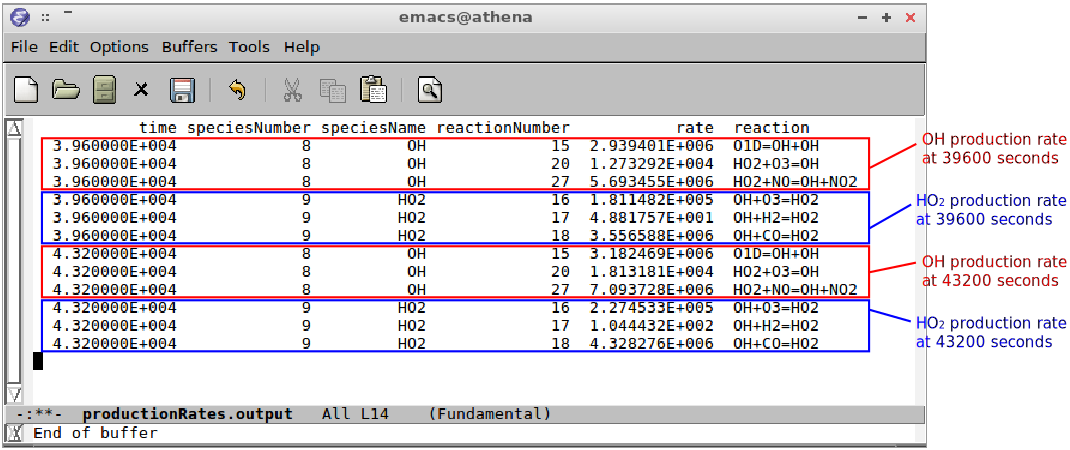
\includegraphics[width=0.95\textwidth]{output-rates.png}
  \caption{Format of the file \texttt{productionRates.output}. The file
    \texttt{lossRates.output} has a similar format.} \label{fig:ropa}
\end{figure}

While the model is running, diagnostic information is printed
to the terminal: this can be redirected to a log file using standard
unix commands. A successfull model run completes with a message
similar to the one shown in Sect.~\ref{sec:install}.
